\documentclass{article}
\renewcommand{\baselinestretch}{1.25}

\usepackage{xeCJK}  % support character

% monokai code
\usepackage{color}
\usepackage{minted}
\usemintedstyle{manni}
\setminted{
    linenos,
    fontsize=\footnotesize,
    resetmargins
}

% insert images
\usepackage{graphicx}
\graphicspath{{images/}{../images/}}
\usepackage{amsmath}
\usepackage{caption}
\numberwithin{figure}{section}
\numberwithin{table}{section}
\numberwithin{listing}{section}
\numberwithin{equation}{section}

\usepackage{subcaption}

% hyperlink
\usepackage{hyperref}
\usepackage{xcolor}
\hypersetup{
    colorlinks,
    linkcolor={red!50!black},
    citecolor={blue!50!black},
    urlcolor={blue!80!black}
}

% auto newline in table
\newcommand{\tabincell}[2]{\begin{tabular}{@{}#1@{}}#2\end{tabular}}
\usepackage{multirow}

\usepackage{mathtools}
\usepackage{amsfonts}

\author{郭一隆(2013011189)}
\title{连连看实验报告}

\begin{document}
    \maketitle

    \tableofcontents
    \newpage

    \listoffigures
    \listoftables
    \renewcommand\listoflistingscaption{List of Source Codes}
    \listoflistings
    \newpage

    \section{原创性} % (fold)
    \label{sec:原创性}
        
        \textbf{本次连连看大作业由本人独立思考完成,如有雷同,纯属巧合。}

    % section 原创性 (end)

    \section{制作自己的连连看} % (fold)
    \label{sec:制作自己的连连看}
    
        \begin{enumerate}
            \item 在\texttt{MATLAB}环境下,设置当前路径为\texttt{linkgame},运行\texttt{linkgame}(打开\href{../linkgame/linkgame.fig}{\texttt{linkgame.fig}}或右键\href{../linkgame/linkgame.p}{\texttt{linkgame.p}}点“运行”),熟悉游戏。

                \begin{figure}[H]
                    \centering
                    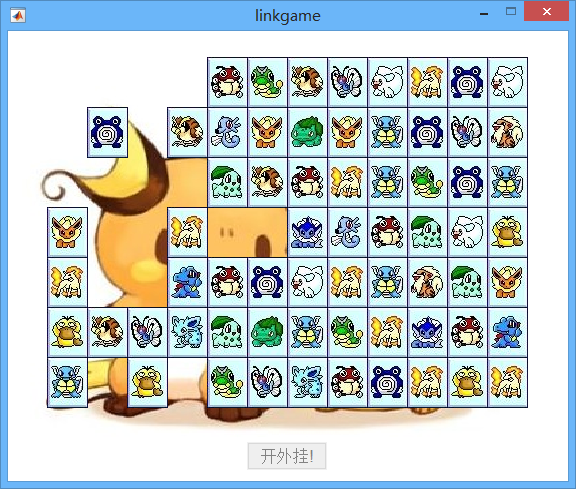
\includegraphics[width=0.8\textwidth]{run_linkgame}
                    \caption{运行连连看}
                \end{figure}

            \item 注意\texttt{linkgame}目录下有个\href{../linkgame/detect.p}{\texttt{detect.p}},它的功能时检测块是否可以消除。现将其删掉,然后把\texttt{linkgame\textbackslash reference}目录下的\href{../linkgame/reference/detect.m}{\texttt{detect.m}}复制到\texttt{linkgame}目录下。\href{../linkgame/detect.m}{\texttt{detect.m}}文件中是\texttt{detect}函数,函数以图像块的索引矩阵与要判断的两个块的下标为输入,如果两个块能消掉则输出\texttt{1},否则输出\texttt{0}。根据文件中的注释提示,实现判断块是否可以消除的功能。写完后再次运行\texttt{linkgame},检验游戏是否仍然可以正确运行。

                算法实现分为以下几个步骤:

                \begin{enumerate}
                    \item \textbf{画十字\texttt{adjcross}}:在给定点周围空白处画十字,遇到块则停止。

                        \begin{listing}[H]
                            \inputminted[firstline=39, lastline=58]{matlab}{../linkgame/detect.m}
                            \caption{\texttt{detect.m(adjcross)}}
                        \end{listing}

                    \item \textbf{判断是否可直连\texttt{canlink0}}:先判断横纵坐标是否在同一直线,再确认路径上是否有障碍。

                        \begin{listing}[H]
                            \inputminted[firstline=61, lastline=72]{matlab}{../linkgame/detect.m}
                            \caption{\texttt{detect.m(canlink0)}}
                        \end{listing}

                    \item \textbf{判断是否可用不超过一个直角的连线连接\texttt{canlink1}}:选取两目标点之一作为起点,画十字;对十字上的点进行遍历,检查是否存在可与另一目标点直连的点。

                        \begin{listing}[H]
                            \inputminted[firstline=75, lastline=96]{matlab}{../linkgame/detect.m}
                            \caption{\texttt{detect.m(canlink1)}}
                        \end{listing}

                    \item \textbf{判断可连性\texttt{canlink2}}:选取两目标点之一作为起点,画十字;对十字上的点进行遍历,检查是否存在可与另一目标用不超过一个直角的连线连接的点。

                        \inputminted[firstline=99, lastline=120]{matlab}{../linkgame/detect.m}
                        \begingroup
                            \captionof{listing}{\texttt{detect.m(canlink2)}}
                        \endgroup
                \end{enumerate}

                再次运行\texttt{linkgame},\href{../linkgame/detect.m}{\texttt{detect.m}}功能正常。

                \begin{minted}{matlab}
function bool = detect(mtx, x1, y1, x2, y2)
    
    [m,n] = size(mtx);
    
    % add surrounding zeros
    mtx = [0,zeros(1,n),0;
        zeros(m,1),mtx,zeros(m,1);
        0,zeros(1,n),0];
    
    origin = mtx(x1+1,y1+1);
    target = mtx(x2+1,y2+1);
    
    if origin == target && canlink2(mtx,x1+1,y1+1,x2+1,y2+1)
        bool = 1;
    else
        bool = 0;
    end
       
end
                \end{minted}
                \begingroup
                    \captionof{listing}{\texttt{detect.m(main)}}
                \endgroup

                \begin{figure}[H]
                    \centering
                    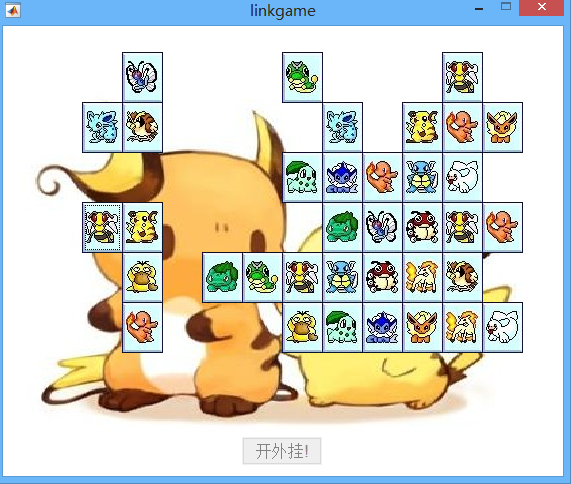
\includegraphics[width=0.8\textwidth]{mydetect_linkgame}
                    \caption{重写\texttt{detect.m}后运行\texttt{linkgame}}
                \end{figure}

        \end{enumerate}

    % section 制作自己的连连看 (end)


\end{document}